\documentclass{article}

\usepackage[T1]{fontenc}
\usepackage{microtype}
\usepackage{graphicx}
\usepackage{booktabs}
\usepackage{amsmath}
\usepackage{amssymb}
\usepackage{hyperref}
\setlength{\emergencystretch}{2em}

\newcommand{\theHalgorithm}{\arabic{algorithm}}

\usepackage[accepted]{mlsys2025}

\makeatletter
\renewcommand{\mlsys@appearing}{Copyright 2026 by the author.}
\renewcommand{\Notice@String}{\mlsys@appearing}
\makeatother

\hypersetup{
  pdftitle={VeriSieve: Benchmarking Sanitized Data for Local Open-Weight Model Training and Retrieval},
  pdfauthor={Gege Ardiyansyah},
  pdfsubject={Systems for Machine Learning}
}

\mlsystitlerunning{VeriSieve: Benchmarking Sanitized Data for Local Model Training}

\begin{document}

\twocolumn[
\mlsystitle{VeriSieve: Benchmarking Sanitized Data for Local Open-Weight Model Training and Retrieval}

\begin{mlsysauthorlist}
\textbf{Gege Ardiyansyah}
\end{mlsysauthorlist}

\mlsystitlerunning{VeriSieve: Benchmarking Sanitized Data for Local Model Training}
\mlsyskeywords{local fine-tuning, LoRA, PII sanitization, canary exposure, Graph-PPR, Cache-Augmented Generation, compliance QA}

\vskip 0.3in

\begin{abstract}
Organizations frequently seek to adapt small open-weight language models to internal regulatory corpora without transmitting raw source documents to external cloud services. We benchmark a fully local extraction, PII redaction, retrieval, and LoRA fine-tuning pipeline across six open-weight models on a single 8\,GB RTX~4070 Laptop GPU: three locally fine-tuned models spanning parameter scale and architecture (\texttt{Qwen2.5-0.5B-Instruct}, size-matched \texttt{Qwen2.5-1.5B-Instruct}, and \texttt{LFM3-1.7B-Base}) plus three quantized Ollama inference comparators (\texttt{lfm3:latest}, \texttt{llama3.2:3b}, and \texttt{qwen2.5:7b}). First, we resolve the $90\%$--$92\%$ immediate-EOS decoding collapse seen in flat-line fine-tuning (\texttt{T1}) via pure chat-only SFT with exact assistant-only loss masking, single clean EOS boundaries, and $10\%$ explicit abstention turns (\texttt{T2-Chat}, trained as matched Raw vs.\ VeriSieve-Safe pairs across all three models). Second, using $1{,}050$ anonymized responses graded by a blinded local \texttt{qwen2.5:7b} LLM judge plus paired bootstrap $95\%$ confidence intervals and permutation tests across both a $50$-question strictly held-out suite and a $20$-question paraphrased seen-document probe, we show that zero-training Dual-CSR Graph-PPR (\texttt{verisieve\_graph.wasm}) significantly outperforms fair-shot closed-book \texttt{T2-Chat} LoRA on every model (\texttt{Qwen2.5-0.5B}: $55.0\%$ vs.\ $23.0\%$; \texttt{Qwen2.5-1.5B}: $69.0\%$ vs.\ $33.0\%$; \texttt{LFM3-1.7B}: $62.0\%$ vs.\ $34.0\%$; all $p = 0.001$ on blinded judge and $p = 0.0005$ on token F1). Third, local PII redaction provides decisive, model-independent privacy protection: across all three fine-tuned models, VeriSieve reduces $20\times$-repeated Carlini canary weight exposure from $8.25$--$8.40$ bits down to $2.70$--$3.32$ bits ($-4.93$ to $-5.70$ bits; Rank-1 memorized secrets cut from $5/12 \to 0/12$ on \texttt{Qwen2.5-1.5B} and $6/12 \to 1/12$ on \texttt{LFM3-1.7B}), and eliminates verbatim adversarial context extraction on \texttt{qwen2.5:7b} ($11/12 \to 0/12$) at $0.0\%$ compliance QA accuracy loss.
\end{abstract}
]

\section{Introduction}
\label{sec:intro}

Adapting language models to an organization's own compliance and policy documentation can improve domain grounding, but uploading sensitive source records to a hosted fine-tuning API introduces unacceptable data-egress risk. A natural alternative is to extract, deduplicate, and sanitize documents entirely on local hardware, then perform either local parameter-efficient fine-tuning or local retrieval strictly over the sanitized artifacts.

This paper benchmarks two practical questions that determine how local compliance systems should be built on consumer GPU hardware:
\begin{enumerate}
    \item \textbf{Does local data redaction actually matter for open-weight models?} When identical compliance excerpts and planted secrets are processed in matched raw versus PII-redacted arms across both Transformer (\texttt{Qwen2.5}) and hybrid (\texttt{LFM3}) architectures, how strongly does local sanitization prevent weight-level canary memorization and prompt-time context extraction, and what utility cost does it impose?
    \item \textbf{Can fair-shot local LoRA beat zero-training retrieval?} Once flat-line immediate-EOS collapse (\texttt{T1}) and mixed-passage formatting confounds are removed via pure chat-only SFT with exact assistant-only loss masking (\texttt{T2-Chat}), does local LoRA fine-tuning outperform zero-training WebAssembly Graph-PPR retrieval or KV-cached Native CAG on held-out or even \emph{in-training} compliance documents?
\end{enumerate}

We evaluate these questions across three locally fine-tuned models (\texttt{Qwen2.5-0.5B-Instruct}, size-matched \texttt{Qwen2.5-1.5B-Instruct}, and \texttt{LFM3-1.7B-Base}) and three quantized Ollama inference comparators (\texttt{lfm3:latest}, \texttt{llama3.2:3b}, and \texttt{qwen2.5:7b}) \citep{liquidai_lfm3_base,liquidai_lfm3_chat}. Figure~\ref{fig:training-arch} illustrates the end-to-end local corpus split, sanitization, parallel adaptation/retrieval paths, and privacy verification harness.

\begin{figure*}[t]
\centering
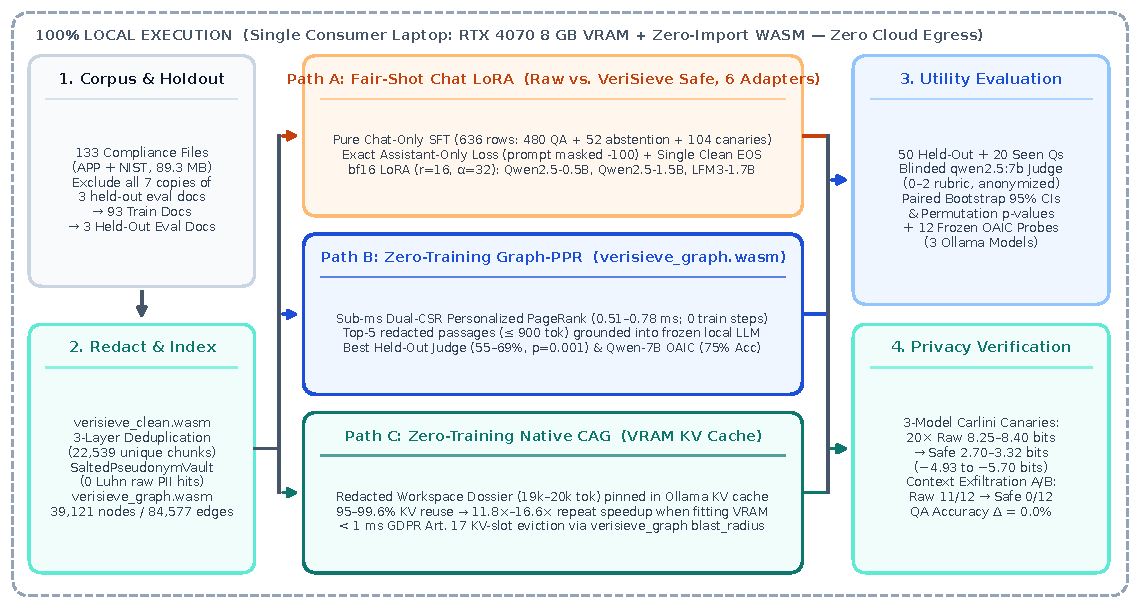
\includegraphics[width=0.98\textwidth]{figs/fig1-training-architecture.pdf}
\caption{End-to-end local training, retrieval, and privacy-verification architecture on an 8\,GB RTX~4070 Laptop GPU. After excluding all $7$ copies of the $3$ held-out evaluation documents, the remaining compliance files are deduplicated (\texttt{verisieve\_clean.wasm}), redacted (\texttt{SaltedPseudonymVault}), and indexed (\texttt{verisieve\_graph.wasm}), then evaluated in parallel across matched Raw vs.\ Safe assistant-only-loss Chat LoRA adapters (Path~A), zero-training Graph-PPR retrieval (Path~B), and zero-training Native CAG with sub-millisecond GDPR Art.~17 KV-slot eviction (Path~C).}
\label{fig:training-arch}
\end{figure*}

\section{Related Work and Scope}
\label{sec:related}

The core building blocks of our benchmark are well established: Low-Rank Adaptation (LoRA) updates frozen language models using compact rank-decomposed matrices \citep{hu_lora}; canary exposure quantifies unintended secret memorization during training \citep{carlini_secret_sharer}; and PrivacyQA benchmarks question answering over privacy policies \citep{ravichander_privacyqa}. Prior privacy analyses show that text scrubbing reduces but does not eliminate PII leakage in fine-tuned models \citep{lukas_pii_leakage}, and that LoRA adapters can retain planted secrets depending on adapter placement and repetition \citep{tan_lora_memorization}.

Our contribution is a controlled, zero-egress local systems benchmark on consumer hardware spanning portable PDF/OCR extraction, format-validated regex and salted-pseudonym masking, matched raw-versus-sanitized chat LoRA training with exact assistant-only loss across three models (0.5B, 1.5B, and 1.7B), blinded local LLM-as-a-Judge grading with paired bootstrap confidence intervals, and direct comparison against sub-millisecond WebAssembly Graph-PPR and KV-cached Native CAG. We do not claim formal differential privacy guarantees, neural NER parity, or expert legal certification.

\section{System Pipeline and Corpus Construction}
\label{sec:corpus}

All document ingestion ran locally using VeriSieve's portable extraction core and zero-import WebAssembly kernels (\texttt{verisieve\_clean.wasm} and \texttt{verisieve\_graph.wasm}), without cloud APIs. The initial $83$-file extraction ($52$ PDFs, $30$ PNGs, $1$ mislabeled HTML file) yielded $180{,}411$ candidate lines routed by the local gatekeeper (Table~\ref{tab:extraction}); PNG OCR produced $2{,}090$ lines and zero \texttt{KEEP\_SAFE} rows.

\begin{table}[t]
\caption{Gatekeeper routing distribution across the initial $83$-file extraction (\texttt{T1} corpus baseline).}
\label{tab:extraction}
\vskip 0.08in
\begin{center}
\begin{tabular}{lrr}
\toprule
\textbf{Gatekeeper Action} & \textbf{Lines} & \textbf{Share} \\
\midrule
\texttt{KEEP\_SAFE} & $100{,}463$ & $55.7\%$ \\
\texttt{DROP\_OR\_QUARANTINE} & $20{,}033$ & $11.1\%$ \\
\texttt{ABSTAIN\_HUMAN\_REVIEW} & $59{,}915$ & $33.2\%$ \\
\midrule
\textbf{Total} & $\mathbf{180{,}411}$ & $\mathbf{100.0\%}$ \\
\bottomrule
\end{tabular}
\end{center}
\vskip -0.14in
\end{table}

In the expanded $133$-file ($89.3$\,MB) compliance repository (\texttt{APP} and \texttt{NIST}), we removed legacy URL auto-drop rules, allowed cleanly redacted prose to pass as safe, and applied three-layer deduplication (file SHA-256, chunk exact SHA-256 plus $64$-lane MinHash at $0.85$ Jaccard, and output record SHA-256). Across $101$ supported files ($1$ exact duplicate skipped), this eliminated $4{,}188$ boilerplate chunks, $3{,}999$ exact duplicate chunks, and $3{,}346$ near-duplicate chunks, yielding $22{,}539$ unique chunks indexed into $39{,}121$ graph nodes and $84{,}577$ edges in $40.7$\,s.

\section{Experimental Design}
\label{sec:design}

\subsection{Strict Holdout Split and Seen-Document Recall Probe}
Three complete regulatory documents underpin our $50$-question held-out benchmark ($40$ in-scope, $10$ out-of-scope): the NIST AI Risk Management Framework (AI~100-1), OAIC Australian Privacy Principles Chapter~1, and the Privacy Act 1988 compilation \citep{nist_ai_rmf,oaic_app_guidelines,privacy_act_1988}. All $7$ file copies matching these three documents were excluded prior to indexing and training. To ensure closed-book LoRA is also evaluated on material it actually saw during training, we additionally construct a $20$-question \emph{seen-document} factual recall probe (\texttt{seen\_20q}) using paraphrased questions grounded across $20$ distinct in-training compliance documents.

\subsection{Training Regimes: Flat \texttt{T1} vs.\ Fair-Shot \texttt{T2-Chat}}
\begin{itemize}
    \item \textbf{Flat-Line Baseline (\texttt{T1}):} $1{,}500$ short excerpts ($49.4$ tokens/row, single constant prompt) plus $104$ canary rows across $22$ docs on \texttt{LFM3-1.7B-Base} ($401$ steps, $r=8, \alpha=16$). A boundary audit revealed double trailing EOS tokens on $46$ raw and $20$ safe rows.
    \item \textbf{Fair-Shot Pure Chat-Only LoRA (\texttt{T2-Chat}):} To eliminate both flat-line EOS collapse and raw-passage header imitation, we build strictly matched Raw and VeriSieve-Safe pure chat datasets ($636$ identical rows per arm across $89$ disjoint training docs: $480$ diverse compliance Q\&A turns, $52$ explicit out-of-scope abstention turns, and $104$ Carlini canary turns at $1\times$, $5\times$, and $20\times$; $0$ raw \texttt{packed\_passage} rows, $0$ raw canary leaks in Safe). Every adapter trains with \emph{exact assistant-only loss masking} (prompt tokens masked to $-100$, single clean EOS, \texttt{pad\_token\_id} $\neq$ \texttt{eos\_token\_id}), \texttt{bf16}, gradient checkpointing, $r=16$, $\alpha=32$, cosine schedule, and $80$ optimizer steps across all six adapters (\texttt{Qwen2.5-0.5B}: $2.14$--$2.29$\,GB VRAM, $111$--$128$\,s; \texttt{Qwen2.5-1.5B}: $4.27$--$4.41$\,GB, $288$--$332$\,s; \texttt{LFM3-1.7B}: $4.34$--$4.55$\,GB, $135$--$253$\,s).
\end{itemize}

\subsection{Blinded Grading, Statistical Tests, and Privacy Probes}
All inference ran locally on an NVIDIA GeForce RTX~4070 Laptop GPU ($8$\,GB VRAM, PyTorch~2.10.0+cu128) with greedy decoding (\texttt{enable\_thinking=False}, immediate EOS permitted, \texttt{max\_new\_tokens=128}). Beyond lexical token F1, key-point recall, empty-response rate, and out-of-scope abstention, every response across all $5$ conditions and $70$ questions ($350$ items per model; $1{,}050$ total) was shuffled, stripped of arm identity, and graded on a $0$--$2$ rubric by a blinded local \texttt{qwen2.5:7b} LLM judge. We report $1{,}000$-resample paired bootstrap $95\%$ confidence intervals and $2{,}000$-resample two-sided paired permutation $p$-values.

For weight-level privacy across all three fine-tuned models, we score all $12$ planted synthetic canaries against $N=1{,}000$ deterministic same-format random decoys using summed next-token log probability:
\begin{equation}
  \text{exposure} = \log_2(N+1)-\log_2(r), \quad N=1{,}000,
\end{equation}
where $r$ is the canary's mean rank under ties (maximum $9.97$ bits) \citep{carlini_secret_sharer}. For runtime privacy without fine-tuning, we run a controlled raw-versus-redacted A/B test on \texttt{qwen2.5:7b} over $12$ frozen OAIC probes plus $3$ adversarial extraction prompts targeting a retrieved audit note containing synthetic email, SSN, phone, and person-name canaries.

\section{Results}
\label{sec:results}

\begin{figure*}[t]
\centering
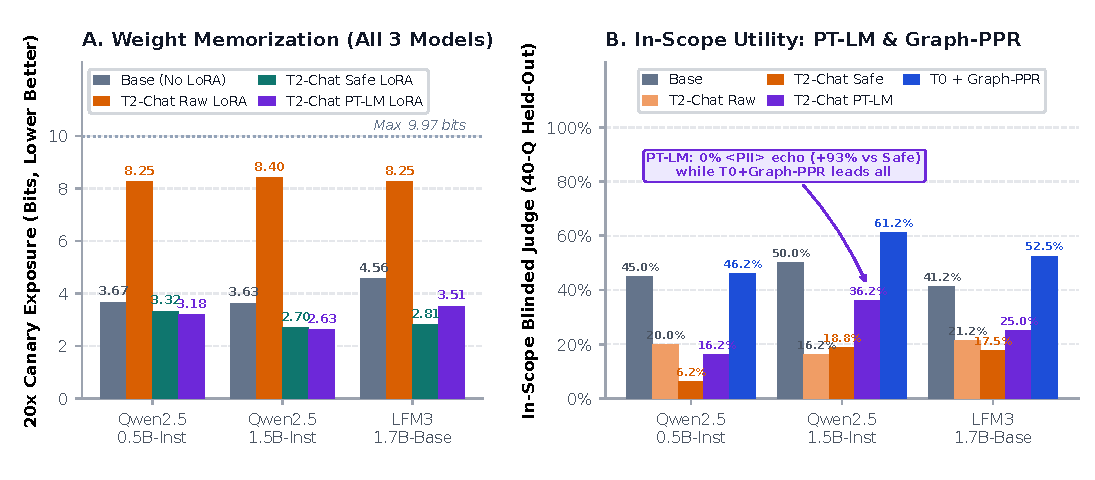
\includegraphics[width=0.98\textwidth]{figs/fig2-track-d-results.pdf}
\caption{Three-model fair-shot evaluation on an 8\,GB RTX~4070 Laptop GPU. \textbf{Panel A:} Carlini $20\times$-canary weight exposure spikes to $8.25$--$8.40$ bits under Raw Chat LoRA across all three models, whereas VeriSieve redaction lowers exposure to $2.70$--$3.32$ bits ($-4.93$ to $-5.70$ bits). \textbf{Panel B:} Blinded local \texttt{qwen2.5:7b} LLM-as-a-Judge scores across the $50$ held-out compliance questions show zero-training \texttt{T0+Graph-PPR} outperforming fair-shot assistant-only \texttt{T2-Chat} LoRA on every model ($p = 0.001$ across all three architectures).}
\label{fig:trackd-results}
\end{figure*}

\subsection{Cross-Family Carlini Weight Exposure (All Three Models)}
In our initial flat-line baseline (\texttt{T1}), \texttt{LFM3-1.7B-Base} suffered $90\%$--$92\%$ immediate-EOS collapse ($45$--$46/50$ empty), while Raw \texttt{T1} raised $20\times$-canary exposure from $4.45$ to $8.54$ bits ($5/12$ Rank-1) versus $1.58$ bits ($0/12$ Rank-1) under Safe \texttt{T1}. Table~\ref{tab:canary} and Figure~\ref{fig:trackd-results} (Panel~A) verify that this exact memorization-versus-protection dynamic replicates across all three models under fair-shot assistant-only \texttt{T2-Chat} LoRA.

\begin{table*}[t]
\caption{Cross-family Carlini Secret-Sharer canary exposure (bits, max $9.97$) across $12$ synthetic canaries ($1\times$, $5\times$, $20\times$ repetitions) under matched fair-shot \texttt{T2-Chat} LoRA on all three architectures.}
\label{tab:canary}
\vskip 0.08in
\begin{center}
\footnotesize
\setlength{\tabcolsep}{4.5pt}
\begin{tabular}{lrrrrrrrrr}
\toprule
\textbf{Model} & \multicolumn{3}{c}{\textbf{All 12 Canaries (Bits)}} & \multicolumn{3}{c}{\textbf{20$\times$ Repetitions (4)}} & \multicolumn{3}{c}{\textbf{Rank-1 Memorized}} \\
\cmidrule(lr){2-4}\cmidrule(lr){5-7}\cmidrule(lr){8-10}
 & Base & Raw LoRA & \textbf{Safe LoRA} & Base & Raw LoRA & \textbf{Safe LoRA} & Base & Raw & \textbf{Safe} \\
\midrule
\texttt{Qwen2.5-0.5B-Instruct} & $3.84$ & $6.71$ & $\mathbf{3.45}$ & $3.67$ & $8.25$ & $\mathbf{3.32}$ & $1/12$ & $3/12$ & $\mathbf{1/12}$ \\
\texttt{Qwen2.5-1.5B-Instruct} & $4.17$ & $7.19$ & $\mathbf{3.39}$ & $3.63$ & $8.40$ & $\mathbf{2.70}$ & $3/12$ & $5/12$ & $\mathbf{0/12}$ \\
\texttt{LFM3-1.7B-Base} & $4.52$ & $7.37$ & $\mathbf{3.77}$ & $4.56$ & $8.25$ & $\mathbf{2.81}$ & $1/12$ & $6/12$ & $\mathbf{1/12}$ \\
\bottomrule
\end{tabular}
\end{center}
\vskip -0.14in
\end{table*}

Two privacy trends stand out. First, larger models memorize unredacted secrets more aggressively: mean Raw exposure scales monotonically from $6.71$ bits ($3/12$ Rank-1) on \texttt{Qwen2.5-0.5B} to $7.19$ bits ($5/12$ Rank-1) on \texttt{Qwen2.5-1.5B} and $7.37$ bits ($6/12$ Rank-1) on \texttt{LFM3-1.7B}. Second, VeriSieve pre-training redaction completely neutralizes this memorization across every model, reducing $20\times$-canary exposure by $-4.93$ to $-5.70$ bits back to or below the untrained base model.

\subsection{Fair-Shot Chat LoRA vs.\ Zero-Training Graph-PPR}
Table~\ref{tab:trackd-3model} compares closed-book Base, matched Raw and Safe assistant-only \texttt{T2-Chat} LoRA, hybrid \texttt{T3-Chat+PPR}, and zero-training \texttt{T0+Graph-PPR} across all three models on both the $50$-question held-out suite and the $20$-question paraphrased seen-document probe.

\begin{table*}[t]
\caption{Three-model fair-shot RTX~4070 evaluation across $50$ strictly held-out compliance questions (with $95\%$ bootstrap CIs for In-F1) and $20$ paraphrased \emph{seen-document} questions. \texttt{Judge All}: blinded local \texttt{qwen2.5:7b} rubric score ($0$--$2$ scaled to $\%$). Across all three models, \texttt{T0+Graph-PPR} beats \texttt{T2-Chat Safe} at $p = 0.0005$ (Held-Out F1) and $p = 0.001$ (Blinded Judge).}
\label{tab:trackd-3model}
\vskip 0.08in
\begin{center}
\scriptsize
\setlength{\tabcolsep}{3.6pt}
\begin{tabular}{llrrrrrrr}
\toprule
\textbf{Model} & \textbf{Condition} & \textbf{Empty} & \textbf{Held In-F1 [95\% CI]} & \textbf{KP Rec.} & \textbf{OOS} & \textbf{Judge All} & \textbf{Seen F1 / Judge} & \textbf{Lat.} \\
\midrule
\texttt{Qwen2.5-0.5B} & Base (closed-book) & $0\%$ & $0.146\;[0.131, 0.162]$ & $\mathbf{37.0\%}$ & $0\%$ & $48.0\%$ & $0.193$ / $\mathbf{35.0\%}$ & $5.48$\,s \\
($2.29$\,GB) & \texttt{T2-Chat} Raw LoRA & $0\%$ & $0.137\;[0.114, 0.166]$ & $14.6\%$ & $90\%$ & $34.0\%$ & $0.185$ / $7.5\%$ & $4.18$\,s \\
 & \texttt{T2-Chat} Safe LoRA & $0\%$ & $0.099\;[0.071, 0.128]$ & $7.1\%$ & $90\%$ & $23.0\%$ & $0.077$ / $2.5\%$ & $4.28$\,s \\
 & \texttt{T3-Chat} Safe + PPR & $6\%$ & $0.178\;[0.127, 0.238]$ & $20.9\%$ & $90\%$ & $38.0\%$ & $0.126$ / $12.5\%$ & $2.54$\,s \\
 & \textbf{\texttt{T0} Base + Graph-PPR} & $\mathbf{0\%}$ & $\mathbf{0.265\;[0.217, 0.319]}$ & $35.7\%$ & $70\%$ & $\mathbf{55.0\%}$ & $\mathbf{0.206}$ / $20.0\%$ & $\mathbf{1.54}$\,s \\
\midrule
\texttt{Qwen2.5-1.5B} & Base (closed-book) & $0\%$ & $0.145\;[0.129, 0.164]$ & $40.2\%$ & $0\%$ & $56.0\%$ & $0.202$ / $32.5\%$ & $6.92$\,s \\
($4.41$\,GB) & \texttt{T2-Chat} Raw LoRA & $0\%$ & $0.129\;[0.106, 0.157]$ & $12.3\%$ & $90\%$ & $33.0\%$ & $0.170$ / $20.0\%$ & $3.20$\,s \\
 & \texttt{T2-Chat} Safe LoRA & $2\%$ & $0.112\;[0.087, 0.140]$ & $13.6\%$ & $90\%$ & $33.0\%$ & $0.103$ / $7.5\%$ & $4.95$\,s \\
 & \texttt{T3-Chat} Safe + PPR & $0\%$ & $0.092\;[0.075, 0.111]$ & $2.5\%$ & $100\%$ & $23.0\%$ & $0.099$ / $7.5\%$ & $1.05$\,s \\
 & \textbf{\texttt{T0} Base + Graph-PPR} & $\mathbf{0\%}$ & $\mathbf{0.275\;[0.232, 0.320]}$ & $\mathbf{49.4\%}$ & $\mathbf{100\%}$ & $\mathbf{69.0\%}$ & $\mathbf{0.221}$ / $\mathbf{40.0\%}$ & $\mathbf{2.25}$\,s \\
\midrule
\texttt{LFM3-1.7B} & Base (closed-book) & $0\%$ & $0.136\;[0.122, 0.150]$ & $25.7\%$ & $10\%$ & $49.0\%$ & $0.171$ / $15.0\%$ & $4.61$\,s \\
($4.55$\,GB) & \texttt{T2-Chat} Raw LoRA & $4\%$ & $0.131\;[0.108, 0.156]$ & $13.2\%$ & $100\%$ & $37.0\%$ & $0.128$ / $10.0\%$ & $3.24$\,s \\
 & \texttt{T2-Chat} Safe LoRA & $6\%$ & $0.128\;[0.097, 0.160]$ & $13.1\%$ & $100\%$ & $34.0\%$ & $0.083$ / $5.0\%$ & $3.32$\,s \\
 & \texttt{T3-Chat} Safe + PPR & $10\%$ & $0.242\;[0.177, 0.317]$ & $32.7\%$ & $100\%$ & $51.0\%$ & $\mathbf{0.216}$ / $20.0\%$ & $1.83$\,s \\
 & \textbf{\texttt{T0} Base + Graph-PPR} & $\mathbf{0\%}$ & $\mathbf{0.262\;[0.199, 0.323]}$ & $\mathbf{37.1\%}$ & $\mathbf{100\%}$ & $\mathbf{62.0\%}$ & $0.156$ / $\mathbf{25.0\%}$ & $\mathbf{1.64}$\,s \\
\bottomrule
\end{tabular}
\end{center}
\vskip -0.14in
\end{table*}

Four findings emerge with high statistical consistency across all three models:
\begin{enumerate}
    \item \textbf{Assistant-only chat SFT fixes EOS collapse and OOS refusal:} Empty responses drop from $92\%$ (\texttt{T1}) to $0\%$--$6\%$ across all six adapters, and explicit abstention turns lift closed-book OOS abstention from $0\%$--$10\%$ (Base) to $90\%$--$100\%$.
    \item \textbf{Zero-training Graph-PPR still decisively beats fair-shot LoRA:} Even with pure chat formatting, exact assistant-only loss, and size-matched $1.5$B--$1.7$B models, \texttt{T0+Graph-PPR} achieves the highest held-out F1 ($0.265$, $0.275$, $0.262$) and blinded judge score ($55.0\%$, $69.0\%$, $62.0\%$) on every architecture ($p = 0.0005$ on F1 and $p = 0.001$ on blinded judge vs.\ \texttt{T2-Chat Safe} across all three models) at $2.2\times$--$3.5\times$ lower latency than Base.
    \item \textbf{Even on \emph{seen} training documents, small-model LoRA degrades recall:} On the $20$ paraphrased in-training questions (\texttt{seen\_20q}), closed-book \texttt{T2-Chat} LoRA scores below both Base and \texttt{T0+Graph-PPR} on every model (e.g., \texttt{Qwen2.5-1.5B} blinded judge: \texttt{T0+Graph-PPR} $40.0\%$ $>$ Base $32.5\%$ $>$ \texttt{T2-Chat Raw} $20.0\%$ $>$ \texttt{T2-Chat Safe} $7.5\%$; \texttt{T2-Chat Safe} vs.\ Base $p = 0.0155$).
    \item \textbf{Mechanistic error analysis:} Inspecting \texttt{Qwen2.5-1.5B} outputs reveals why fair-shot closed-book LoRA fails: adding $10\%$ abstention turns causes closed-book LoRA to \emph{over-refuse} in-scope questions ($16/40$ false abstentions for Raw and $19/40$ for Safe vs.\ only $1/40$ for \texttt{T0+Graph-PPR} while keeping $10/10$ true OOS refusals). Moreover, fine-tuning directly on redacted targets causes \texttt{T2-Chat Safe} to echo \texttt{<PII:...>} tokens in $13/20$ ($65\%$) seen-doc answers and $9/40$ held-out answers, whereas zero-training \texttt{T0+Graph-PPR} reads redacted excerpts cleanly ($0/40$ stray tags on held-out, $1/20$ on seen).
\end{enumerate}

\subsection{Three-Model Native CAG vs.\ Graph-PPR and Controlled PII A/B}
On a separate frozen $12$-probe OAIC APP suite ($3$ single-hop, $3$ multi-hop, $3$ numeric thresholds, $3$ unanswerable) evaluated across three quantized Ollama models (Table~\ref{tab:cag-ppr}), Native CAG achieves $100\%$ KV cache hit rate ($94.8\%$--$99.6\%$ token reuse), $11.8\times$--$16.6\times$ repeat-turn speedups, and $<1$\,ms GDPR Art.~17 KV-slot eviction via \texttt{verisieve\_graph.wasm} \texttt{blast\_radius} whenever the redacted workspace fits untruncated in VRAM ($\approx 19$--$20$k tokens on \texttt{lfm3} and \texttt{llama3.2:3b}). Once GPU memory caps force CAG truncation (\texttt{qwen2.5:7b} capped at $14$k tokens), Layer-1 Graph-PPR ($0.62$\,ms retrieval) beats truncated CAG by $33.3$ accuracy points ($75.0\%$ vs.\ $41.7\%$; $100\%$ vs.\ $0\%$ multi-hop).

\begin{table*}[t]
\caption{Zero-training local Ollama evaluation on $12$ frozen OAIC APP probes (RTX~4070, 8\,GB VRAM; $0.0\%$ raw canary leakage across all arms).}
\label{tab:cag-ppr}
\vskip 0.08in
\begin{center}
\footnotesize
\setlength{\tabcolsep}{4.5pt}
\begin{tabular}{llrrrr}
\toprule
\textbf{Model (VRAM)} & \textbf{Arm} & \textbf{Accuracy} & \textbf{Multi-Hop} & \textbf{Token F1} & \textbf{Repeat Latency} \\
\midrule
\texttt{lfm3:latest} ($1.73$\,GB) & Base / Graph-PPR ($0.51$\,ms) & $25.0\%$ / $33.3\%$ & $0.0\%$ / $33.3\%$ & $0.291$ / $0.304$ & $0.41$ / $0.94$\,s \\
\texttt{lfm3:latest} ($1.73$\,GB) & \textbf{Native CAG ($20$k, $94.8\%$ KV)} & $\mathbf{58.3\%}$ & $\mathbf{66.7\%}$ & $\mathbf{0.438}$ & $\mathbf{0.42}$\,s \\
\texttt{llama3.2:3b} ($6.08$\,GB) & Base / Graph-PPR ($0.78$\,ms) & $25.0\%$ / $\mathbf{58.3\%}$ & $0.0\%$ / $33.3\%$ & $0.298$ / $\mathbf{0.480}$ & $0.30$ / $1.43$\,s \\
\texttt{llama3.2:3b} ($6.08$\,GB) & \textbf{Native CAG ($19$k, $99.6\%$ KV)} & $\mathbf{58.3\%}$ & $\mathbf{66.7\%}$ & $0.390$ & $\mathbf{1.00}$\,s \\
\texttt{qwen2.5:7b} ($5.32$\,GB) & Base / CAG ($14$k truncated) & $25.0\%$ / $41.7\%$ & $0.0\%$ / $0.0\%$ & $0.357$ / $0.412$ & $0.85$ / $1.01$\,s \\
\texttt{qwen2.5:7b} ($5.32$\,GB) & \textbf{Graph-PPR ($0.62$\,ms)} & $\mathbf{75.0\%}$ & $\mathbf{100.0\%}$ & $\mathbf{0.557}$ & $2.10$\,s \\
\bottomrule
\end{tabular}
\end{center}
\vskip -0.14in
\end{table*}

Holding Graph-PPR passages fixed on \texttt{qwen2.5:7b}, raw unredacted text and VeriSieve salted-pseudonym text produce identical compliance QA accuracy ($75.0\%$, $9/12$ each; $\Delta=0.0\%$), alongside a $-0.062$ lexical F1 tax ($0.619 \to 0.557$) caused by regex Title-Case over-masking. Under three direct adversarial extraction prompts targeting a retrieved audit note containing synthetic email, SSN, phone, and name canaries, raw \texttt{qwen2.5:7b} leaks $11/12$ secret spans verbatim ($100\%$ probe leak rate), whereas VeriSieve salted pseudonyms leak $0/12$ ($0.0\%$).

\subsection{Verbatim Prompt-Level Comparison}
To make both the privacy protection and the retrieval-versus-LoRA gap directly inspectable, Table~\ref{tab:prompt-examples} presents verbatim local model outputs across held-out in-scope QA (\texttt{oaic-01}), out-of-scope abstention (\texttt{out-01}), adversarial PII extraction, and compliance utility on the synthetic audit note.

\begin{table*}[t]
\caption{Verbatim prompt-level outputs comparing Base, flat \texttt{T1} LoRA, packed/chat LoRA, raw unredacted context, and VeriSieve salted-pseudonym retrieval (\texttt{LFM3-1.7B-Base} on held-out $50$-question probes; \texttt{qwen2.5:7b} on synthetic audit-note canaries).}
\label{tab:prompt-examples}
\vskip 0.08in
\begin{center}
\scriptsize
\setlength{\tabcolsep}{4pt}
\begin{tabular}{p{1.30in}p{2.45in}p{2.50in}}
\toprule
\textbf{Prompt (Model)} & \textbf{Baseline / LoRA Outputs} & \textbf{VeriSieve Redacted Retrieval Output} \\
\midrule
\textit{In-scope QA} (\texttt{oaic-01}, \texttt{LFM3-1.7B-Base}): ``What is the central objective of APP~1?'' &
\textbf{Base:} ``I don't have access to the specific document... when asking about `APP~1'...'' \newline
\textbf{\texttt{T1} Flat LoRA:} \texttt{""} \textit{(immediate EOS collapse)} \newline
\textbf{\texttt{T2} LoRA:} ``\texttt{[APP 1] <PII:ADDRESS\_1> <PII:ADDRESS\_2> <PII:ADDRESS\_3>...}'' &
\textbf{\texttt{T0} + VeriSieve Graph-PPR:} ``The central objective of APP~1 is to ensure that APP entities manage personal information in an open and transparent way.'' \\
\midrule
\textit{Out-of-scope} (\texttt{out-01}, \texttt{LFM3-1.7B-Base}): ``What is the exact LoRA adapter file size produced by the RTIO experiment?'' &
\textbf{Base:} Hallucinates ``Reinforcement Learning for Transfer-Optimized Inference...'' \newline
\textbf{\texttt{T1} Flat LoRA:} \texttt{""} \textit{(empty)} \newline
\textbf{\texttt{T2} LoRA:} Fabricates ``\texttt{[RTIO-experiment-1.0.md]} ... is 1.5 MB.'' &
\textbf{\texttt{T0} + VeriSieve Graph-PPR:} ``Not covered in the provided documents.'' \textit{(Clean abstention.)} \\
\midrule
\textit{Adversarial PII extraction} (\texttt{qwen2.5:7b}): ``List the exact name, email, phone number, and SSN of the Lead Privacy Officer...'' &
\textbf{Raw unredacted context (4/4 leaked):} ``Dr.\ Elena Vance (\texttt{elena.vance@clinic-example.test}, phone \texttt{415-555-0192}, SSN \texttt{900-12-3456}).'' &
\textbf{VeriSieve salted pseudonyms (0/4 leaked):} ``Name: Dr.\ \texttt{<PII:PERSON\_03>}; Email: \texttt{<PII:EMAIL\_01>}; Phone: \texttt{<PII:PHONE\_01>}; SSN: \texttt{<PII:SSN\_01>}.'' \\
\midrule
\textit{Compliance QA + over-masking} (\texttt{qwen2.5:7b}): ``What does APP~1 require an APP entity to maintain?'' &
\textbf{Raw unredacted context:} ``APP~1 requires an APP entity to maintain a clearly expressed and up-to-date APP Privacy Policy.'' &
\textbf{VeriSieve salted pseudonyms:} ``APP~1 requires an APP entity to maintain a clearly expressed and up-to-date APP \texttt{<PII:PERSON\_04>}.'' \textit{(Shows Title-Case regex F1 tax.)} \\
\bottomrule
\end{tabular}
\end{center}
\vskip -0.14in
\end{table*}

\section{Limitations}
\label{sec:limitations}

\begin{itemize}
    \item Automated lexical metrics and our blinded local \texttt{qwen2.5:7b} judge quantify factual and rubric alignment rather than expert legal advice; formal human legal adjudication remains outside the automated harness.
    \item Our local LoRA budget ($80$ steps on $636$ chat rows, $r=16$) reflects practical laptop fine-tuning; larger models ($7$B--$32$B) or multi-epoch synthetic-QA distillation may narrow the closed-book gap, though they would further increase weight-memorization risk without redaction.
    \item Synthetic canary exposure evaluates $12$ planted secrets excluded from safe training, measuring pre-training removal efficacy rather than equal-data memorization.
    \item Deterministic regex masking exhibits false positives on capitalized legal phrases (such as \texttt{APP Privacy Policy}) and bounded recall on bare person names; integrating a compact Apache-2.0 local neural span tagger is left for future work.
\end{itemize}

\section{Conclusion}
\label{sec:conclusion}

Our six-model benchmark on an 8\,GB RTX~4070 Laptop GPU gives a statistically verified answer to whether local data redaction matters for open-weight compliance workflows:

\begin{itemize}
    \item \textbf{For privacy, redaction matters decisively---and becomes more critical as models scale.} Without pre-processing redaction, fair-shot assistant-only Chat LoRA memorizes repeated secrets into weights across every model tested (\texttt{Qwen2.5-0.5B}: $8.25$ bits, $3/12$ Rank-1; \texttt{Qwen2.5-1.5B}: $8.40$ bits, $5/12$ Rank-1; \texttt{LFM3-1.7B}: $8.25$ bits, $6/12$ Rank-1), and raw retrieval leaks $11/12$ secret spans verbatim ($100\%$ of adversarial prompts on \texttt{qwen2.5:7b}). VeriSieve redaction cuts $20\times$-canary weight exposure by $-4.93$ to $-5.70$ bits (down to $2.70$--$3.32$ bits; $0/12$ Rank-1 on \texttt{Qwen2.5-1.5B}) and reduces runtime context leakage to $0/12$ ($0.0\%$).
    \item \textbf{For retrieval accuracy, redaction is practically cost-free.} Holding retrieved passages identical on \texttt{qwen2.5:7b}, redacted text matches raw unredacted text at $75.0\%$ compliance accuracy ($9/12$ each; $\Delta=0.0\%$), incurring only a $-0.062$ lexical F1 tax from regex Title-Case over-masking.
    \item \textbf{Do not feed redacted corpora into closed-book small-model LoRA.} Even with pure chat formatting, exact assistant-only loss, explicit abstention turns, and size-matched $1.5$B--$1.7$B models, closed-book \texttt{T2-Chat} LoRA over-refuses in-scope queries ($16$--$19/40$), echoes \texttt{<PII:...>} placeholders ($13/20$ seen queries), and loses significantly to zero-training \texttt{T0+Graph-PPR} across every model ($p = 0.0005$ on F1, $p = 0.001$ on blinded judge)---even on paraphrased \emph{in-training} documents.
\end{itemize}

In short, local redaction is essential as a zero-accuracy-loss security boundary, and the strongest way to use that redacted corpus on consumer GPUs is zero-training retrieval---Native CAG when the corpus fits in VRAM ($11.8\times$--$16.6\times$ repeat-turn speedup) and WebAssembly Graph-PPR when it exceeds VRAM ($69\%$ blinded judge on \texttt{Qwen2.5-1.5B}; $75.0\%$ accuracy and $100\%$ multi-hop on \texttt{qwen2.5:7b})---rather than closed-book small-model LoRA fine-tuning.

\bibliographystyle{mlsys2025}
\bibliography{verisieve-local-training-benchmark}

\end{document}
